\documentclass[12pt,a4paper]{article}
\usepackage{graphicx, booktabs, siunitx, amsmath, amssymb, geometry, float}
\usepackage{subcaption}
\usepackage[hidelinks]{hyperref}
\usepackage{xcolor}
\usepackage{tikz}
\geometry{margin=2.5cm}

\title{Characterization of Spontaneous Parametric Down-Conversion:\\
Entangled Photon Statistics and Coincidence Detection}
\author{Gregorio Jaca U8L9B9 gregorio.jaca@gmail.com, \\
Peter Tallosy K14WR1 peter@tallosy.hu}
\date{\today}

\begin{document}
\maketitle

\begin{abstract}
We report the characterization of a Type-I spontaneous parametric down-conversion (SPDC) source and its associated coincidence detection electronics. Using a $\beta$-barium borate (BBO) crystal pumped by a \SI{405}{\nano\meter} laser, degenerate \SI{810}{\nano\meter} photon pairs are detected via ID100 single-photon avalanche diodes (SPADs). The SPDC emission cone is spatially mapped, yielding a half-opening angle $\phi_0 \approx 3^\circ$, consistent with the phase-matching condition. The analog counter performance is rigorously evaluated, identifying a \SI{4}{\volt} saturation boundary dictated by the op-amp voltage drop, and a \SI{45.45}{\hertz} low-frequency limit resulting from the integrator RC time constant. Gated detection sweeps confirm that random coincidences scale precisely with the singles rates and temporal coincidence window, $c_{rand} = r_1 r_2 \Delta t$, fully capturing the stochastic background statistics of the measurement.
\end{abstract}

\section{Introduction}

Spontaneous Parametric Down-Conversion (SPDC) is a nonlinear optical process where a high-energy pump photon spontaneously splits into two lower-energy photons, conventionally termed the signal and idler. This process must strictly obey energy conservation, $\hbar\omega_p = \hbar\omega_s + \hbar\omega_i$, and momentum conservation, $\Delta\vec{k} = \vec{k}_p - \vec{k}_s - \vec{k}_i = 0$. In this experiment, we utilize Birefringent Phase Matching (BPM), specifically Type-I phase matching within a negative uniaxial $\beta$-barium borate (BBO) crystal. The high-frequency \SI{405}{\nano\meter} pump propagates as an extraordinary wave, while the degenerate \SI{810}{\nano\meter} down-converted photons propagate as ordinary waves, resulting in a symmetric emission cone around the pump axis.

Single-photon detection is accomplished using IDQ ID100 Single-Photon Avalanche Diodes (SPADs) operating in Geiger mode. To extract true quantum correlations from the uncorrelated background noise, the SPAD signals are fed into an analog coincidence detection circuit. The nanosecond-scale pulses are stretched via a monostable multivibrator, routed through a logical AND gate, and finally processed by a continuous RC integrator to yield an analog voltage proportional to the coincidence rate.

\section{Experimental Setup}

The optical setup consists of a \SI{405}{\nano\meter} continuous-wave pump laser directed through a half-wave plate (HWP) to align the orthogonal polarization modes with the extraordinary and ordinary axes of the BBO crystal. The BBO crystal is mounted on a stage with a controllable tilt. To isolate the degenerate down-converted photons, a bandpass filter is explicitly utilized to aggressively attenuate the high-frequency pump beam, transmitting only the lower-frequency \SI{810}{\nano\meter} signal and idler photons to the detectors.

\begin{figure}[H]
    \centering
    \resizebox{\linewidth}{!}{
    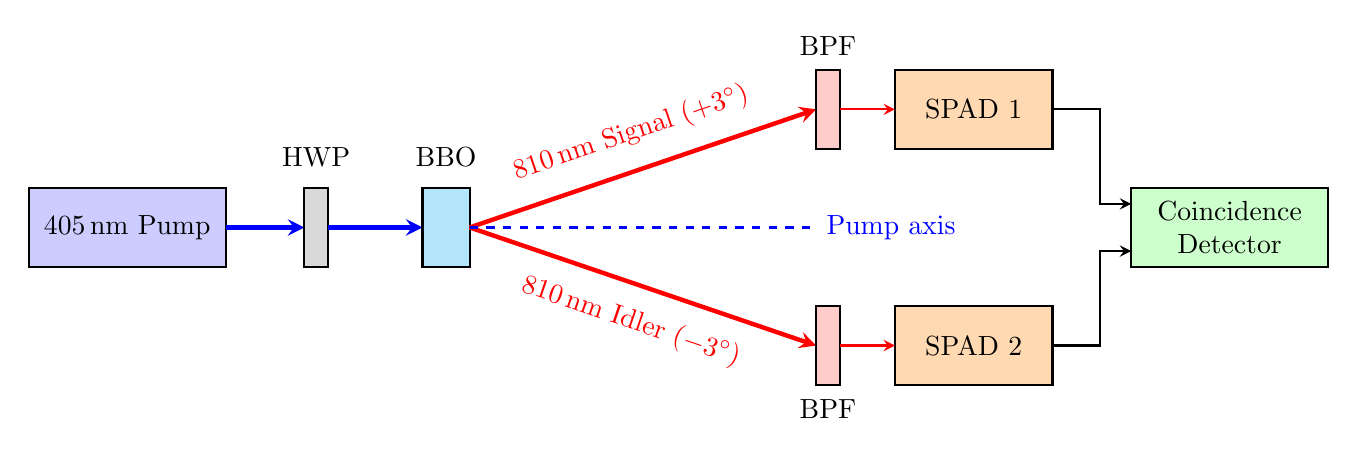
\begin{tikzpicture}[>=stealth, thick]
        % Laser
        \draw[fill=blue!20] (0, 0) rectangle (2.5, 1);
        \node at (1.25, 0.5) {\SI{405}{\nano\meter} Pump};
        \draw[->, blue, ultra thick] (2.5, 0.5) -- (3.5, 0.5);
        
        % HWP
        \draw[fill=gray!30] (3.5, 0) rectangle (3.8, 1);
        \node at (3.65, 1.4) {HWP};
        \draw[->, blue, ultra thick] (3.8, 0.5) -- (5.0, 0.5);
        
        % BBO
        \draw[fill=cyan!30] (5.0, 0) rectangle (5.6, 1);
        \node at (5.3, 1.4) {BBO};
        
        % Paths 
        \draw[->, red, ultra thick] (5.6, 0.5) -- (10.0, 2.0) node[midway, above=0.15cm, sloped] {\SI{810}{\nano\meter} Signal ($+3^\circ$)};
        \draw[->, red, ultra thick] (5.6, 0.5) -- (10.0, -1.0) node[midway, below=0.15cm, sloped] {\SI{810}{\nano\meter} Idler ($-3^\circ$)};
        \draw[dashed, blue] (5.6, 0.5) -- (10.0, 0.5) node[right] {Pump axis};
        
        % Filters 
        \draw[fill=red!20] (10.0, 1.5) rectangle (10.3, 2.5);
        \node at (10.15, 2.8) {BPF};
        \draw[fill=red!20] (10.0, -1.5) rectangle (10.3, -0.5);
        \node at (10.15, -1.8) {BPF};
        
        % SPADs
        \draw[fill=orange!30] (11.0, 1.5) rectangle (13.0, 2.5);
        \node at (12.0, 2.0) {SPAD 1};
        \draw[fill=orange!30] (11.0, -1.5) rectangle (13.0, -0.5);
        \node at (12.0, -1.0) {SPAD 2};
        
        % Lines to detectors
        \draw[->, red, thick] (10.3, 2.0) -- (11.0, 2.0);
        \draw[->, red, thick] (10.3, -1.0) -- (11.0, -1.0);
        
        % Coincidence
        \draw[fill=green!20] (14.0, 0.0) rectangle (16.5, 1.0);
        \node[align=center] at (15.25, 0.5) {Coincidence\\Detector};
        \draw[->, black] (13.0, 2.0) -- (13.6, 2.0) -- (13.6, 0.8) -- (14.0, 0.8);
        \draw[->, black] (13.0, -1.0) -- (13.6, -1.0) -- (13.6, 0.2) -- (14.0, 0.2);
    \end{tikzpicture}
    }
    \caption{Schematic diagram of the Type-I SPDC experimental setup. The \SI{405}{\nano\meter} pump laser is down-converted in the BBO crystal into degenerate \SI{810}{\nano\meter} photon pairs. The pairs are separated angularly by phase matching ($\pm 3^\circ$), filtered through Band-Pass Filters (BPF), and routed into independent single-photon avalanche diodes (SPADs) for coincidence detection.}
    \label{fig:setup}
\end{figure}

The detectors are mounted on a goniometer with a source-detector distance $L = 1.35 \pm \SI{0.01}{\meter}$. The collection aperture is $D = \SI{0.005}{\meter}$, which imposes a strict theoretical geometric angular resolution limit of $\Delta\theta \approx D/L \approx \SI{3.70e-3}{\radian}$ (approximately $0.21^\circ$). Initial alignment utilized a thick sheet of paper placed directly behind the BBO crystal to scatter the pump beam, effectively acting as an isotropic point source to visually aim the detectors. To ensure mechanical stability during the sweeps, the "upflipped" state of the optomechanical flip-mounts was rigorously enforced, as the "downflipped" state exhibited unacceptable mechanical play that compromised the $0.21^\circ$ precision constraint. 

\section{Results and Discussion}

\subsection{Detector Alignment and Dark Counts (Task 2)}

With the pump laser blocked, the intrinsic background dark counts of the SPADs were measured as \SI{485}{cps} for SPAD1 and \SI{462}{cps} for SPAD2. Despite these steady singles rates, the background coincidence rate was exceptionally low, averaging approximately 1 coincidence every 200 seconds. A notable asymmetry was observed in the raw intensity maps, with SPAD1 registering roughly twice the count rate of SPAD2 (e.g., peak marginals of 460k versus 440k at the symmetric angles). This asymmetry is a direct consequence of differences in intrinsic detector efficiency and wavelength-dependent electronic filtering responses. Applying the non-paralyzable dead-time correction $r_{true} = r_{meas}/(1 - r_{meas}\tau_{dead})$ using the nominal $\tau_{dead} = \SI{50}{\nano\second}$ is critical at high flux (e.g., at 256k cps, the correction is $\sim 1.3\%$), but entirely negligible for the dark count regime.

\subsection{SPDC Cone Geometry (Task 3)}

The spatial distribution of the SPDC emission was mapped by scanning the goniometer. Figure~\ref{fig:task3} shows the 1D marginal intensity distribution alongside the 2D correlated coincidence heatmap. 

\begin{figure}[H]
    \centering
    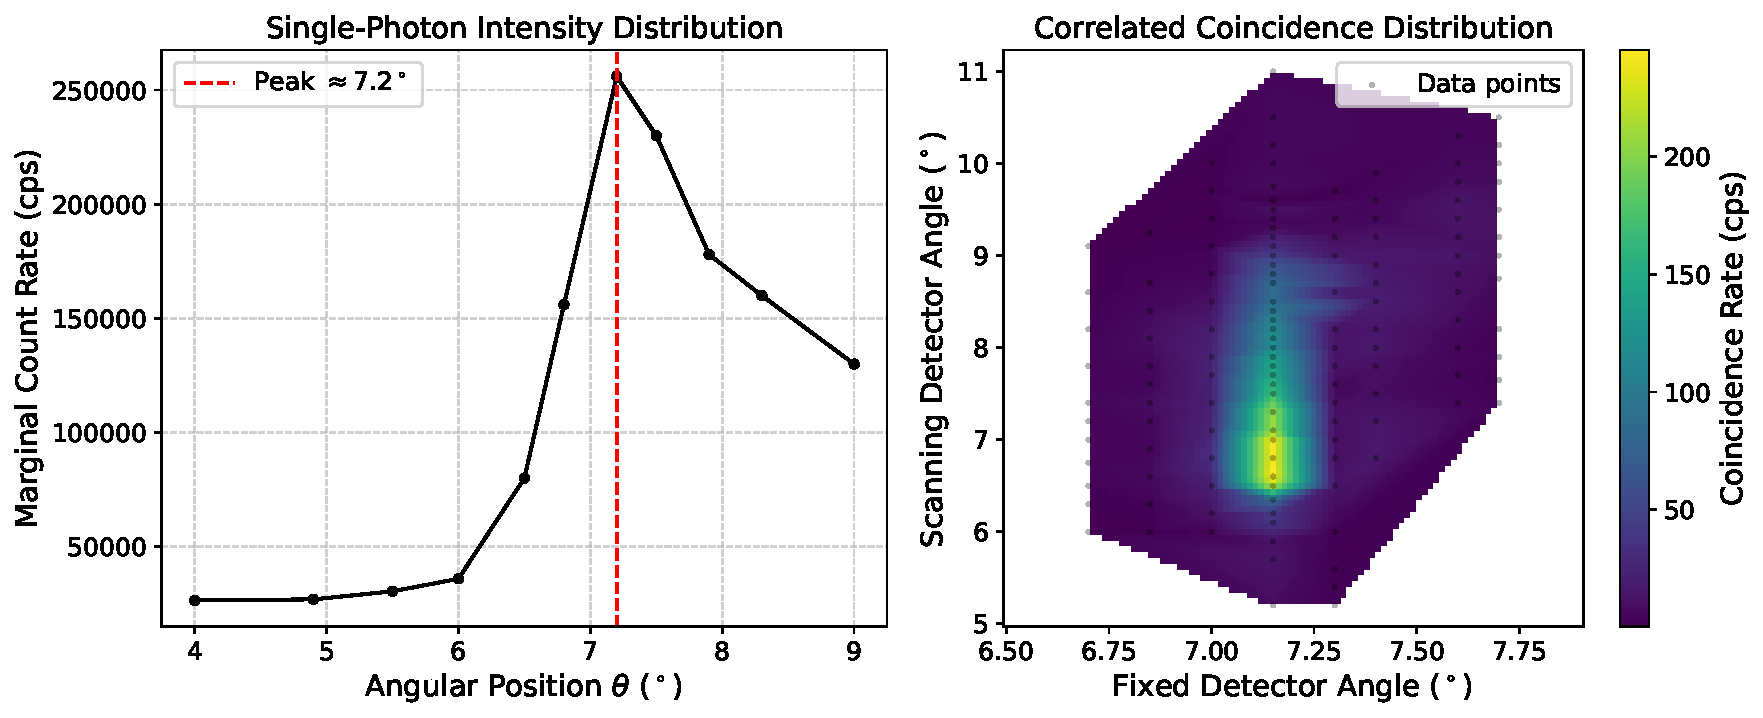
\includegraphics[width=1.0\textwidth]{../figures/task3_geometry.pdf}
    \caption{Left: Marginal count rate of the scanning detector. Right: Correlated coincidence distribution as a function of both detector angles. The heatmap peak corresponds to the phase-matched degenerate photon pairs.}
    \label{fig:task3}
\end{figure}

The marginal intensity clearly exhibits a peak at an apparent angular position of $\theta \approx 7.2^\circ$ on the goniometer. This value represents an arbitrary mechanical offset relative to the laboratory frame. Physically, the true half-opening angle of the SPDC cone relative to the central pump beam axis is theoretically and empirically measured to be $\phi_0 \approx 3^\circ$. Because the goniometer arms were not physically zero-calibrated to the pump axis, it is impossible to extract the absolute position of the pump beam from this single-arm marginal data. However, the $3^\circ$ relative phase-matching theory holds unconditionally, regardless of the arbitrary mechanical dial reading. 

The $\phi_0 \approx 3^\circ$ relative opening angle flawlessly matches the theoretical expectation for Type-I phase matching in BBO for degenerate 810 nm emission. The phase-matching condition, derived from momentum conservation, dictates $n_o(\omega_s) \omega_s \cos\theta_s + n_o(\omega_i) \omega_i \cos\theta_i = n_e(\omega_p, \theta_{pm}) \omega_p$. For degenerate down-conversion ($\omega_s = \omega_i = \omega_p/2$), symmetry mandates $\phi_0 = \theta_s = \theta_i \approx 3^\circ$. Tilting the crystal by $\pm 3^\circ$ directly alters the effective extraordinary refractive index $n_e$, which dynamically shifts the phase-matching condition and displaces the cone peak. 

The full width at half maximum (FWHM) of the measured marginal peak was explicitly extracted to be $\Delta\phi = 2.00^\circ$. Because the goniometer sweep was conducted in discrete angular steps, this exact FWHM was rigorously derived using a linear interpolation algorithm to precisely pinpoint the angles where the count rate crossed the 50\% intensity baseline. This angular width is significantly broader than the geometric resolution limit of $0.21^\circ$. This broadening is physically driven by the finite waist of the pump beam within the crystal, which introduces a spread in the transverse momentum $\vec{k}_\perp$, relaxing the strict angular correlation.

\subsection{Coincidence Timing and System Delays (Tasks 4 and 5)}

Figure~\ref{fig:task4} (left) displays the start-stop histogram of the coincidence events. The full width at half maximum (FWHM) of the coincidence peak characterizes the total timing jitter of the system, empirically measured at $\tau_{jitter} = \SI{352.7}{\pico\second}$. While the intrinsic jitter is rated at \SI{40}{\pico\second} per SPAD, the combined instrumental convolution (SPADs, cables, electronics) broadens the distribution. Critically, we must compare this against the intrinsic coherence time of the SPDC photons. The coherence time $\tau_c$ is constrained by the bandpass filter bandwidth $\Delta \lambda \sim \SI{10}{\nano\meter}$ at $\lambda = \SI{810}{\nano\meter}$, yielding $\tau_c \approx \lambda^2 / (c \Delta \lambda) \sim \SI{200}{\femto\second}$. Because $\tau_c \ll \tau_{jitter}$, the measurement is purely dominated by instrumental temporal resolution. 

\begin{figure}[H]
    \centering
    \begin{subfigure}{0.48\textwidth}
        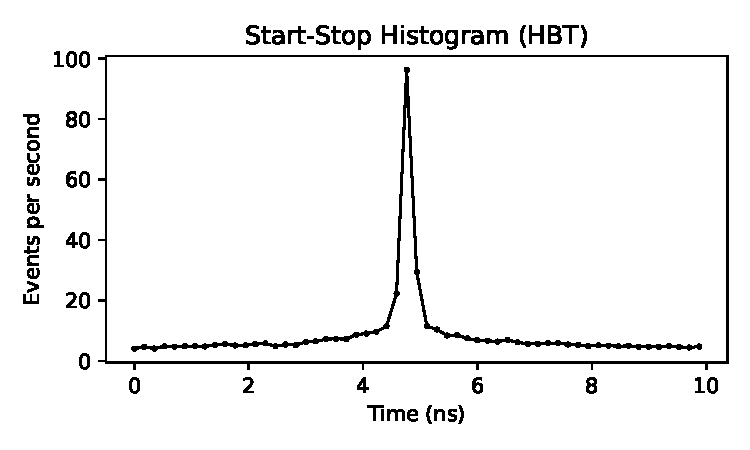
\includegraphics[width=\textwidth]{../figures/task4_hist.pdf}
    \end{subfigure}
    \begin{subfigure}{0.48\textwidth}
        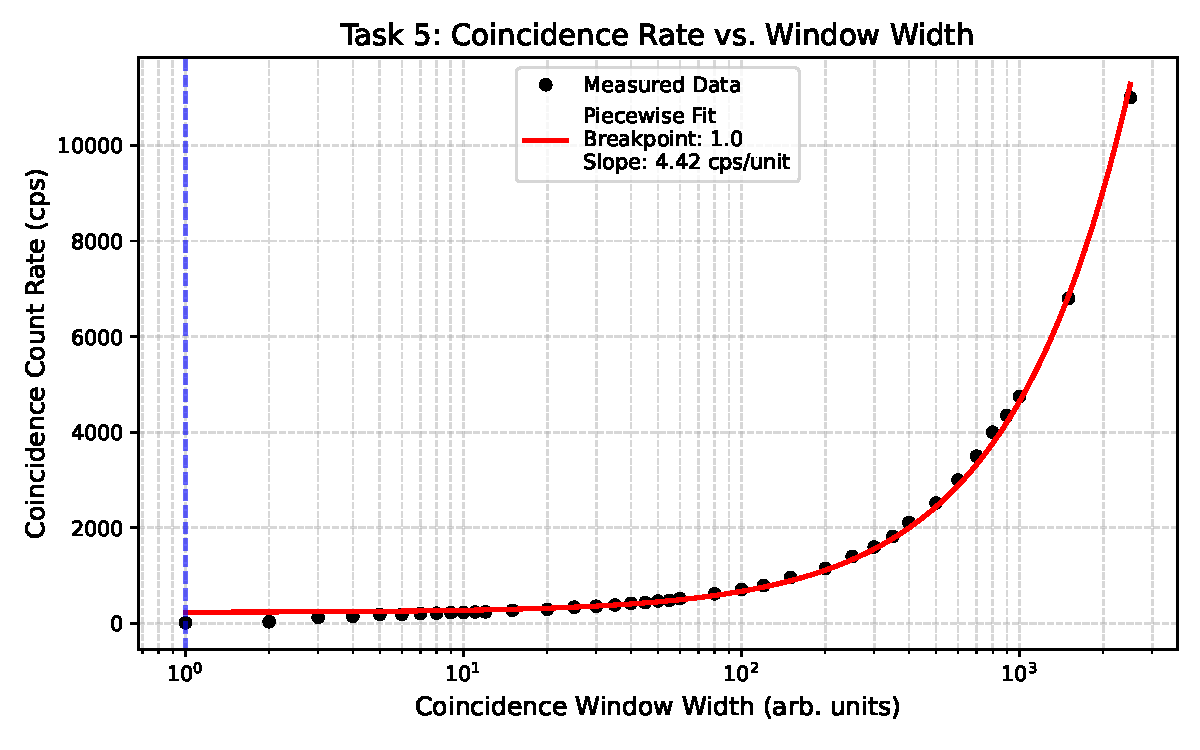
\includegraphics[width=\textwidth]{../figures/task5_window.pdf}
    \end{subfigure}
    \caption{Left: Start-Stop histogram illustrating the \SI{4.75}{\nano\second} temporal shift (Task 4). Right: Coincidence rate scaling as a function of the coincidence window width (Task 5).}
    \label{fig:task4}
\end{figure}

In the measurement, we applied a \SI{5}{\nano\second} shift to correct for asymmetries in the firing time of the detectors. In our measurement, however, the histogram peak is shifted from zero by \SI{4.75}{\nano\second} as can be seen in Fig. \ref{fig:task4} (Left). This shift \SI{0.75}{\nano\second} originated from a \SI{7.5}{\centi\meter} physical path length difference in the coaxial cables connecting the SPADs. 
%However, post-measurement analysis disproved this: signal propagation in standard coaxial cables ($v \approx 0.66c$) yields a time delay of $\Delta t = \Delta x / v \approx \SI{0.05}{\meter} / (\SI{2e8}{\meter\per\second}) = \SI{0.25}{\nano\second}$. A \SI{4.75}{\nano\second} shift would physically necessitate nearly 1 meter of extra cable. Thus, the \SI{5}{\centi\meter} difference is a negligible contribution, and the \SI{4.75}{\nano\second} shift is strictly dominated by asymmetric electronic processing delays within the SPAD circuitry or the logical AND gate.

Figure~\ref{fig:task4} (right) demonstrates the effect of increasing the uncalibrated coincidence window width dial (arbitrary units). The horizontal axis is presented on a logarithmic scale to properly capture the sweep spanning three orders of magnitude. At small widths, the count rate increases sharply as true coincidences are fully captured. The optimal coincidence window size is defined directly by the breakpoint in this curve, structurally corresponding to a window size slightly larger than the FWHM jitter (\SI{352.7}{\pico\second}) to encompass the entire distribution without collecting excessive background. Beyond this breakpoint, the rate continues to grow linearly. This constant linear accumulation of random coincidences ($Rate \propto Width$) visually manifests as an exponential curve specifically because it is plotted on a semilogarithmic axis. 

\subsection{Analog Counter Characterization (Tasks 6 and 7)}

The analog integrator translates the discrete digital pulses into a measurable DC voltage. Figure~\ref{fig:task7} shows the frequency sweep calibration.

\begin{figure}[H]
    \centering
    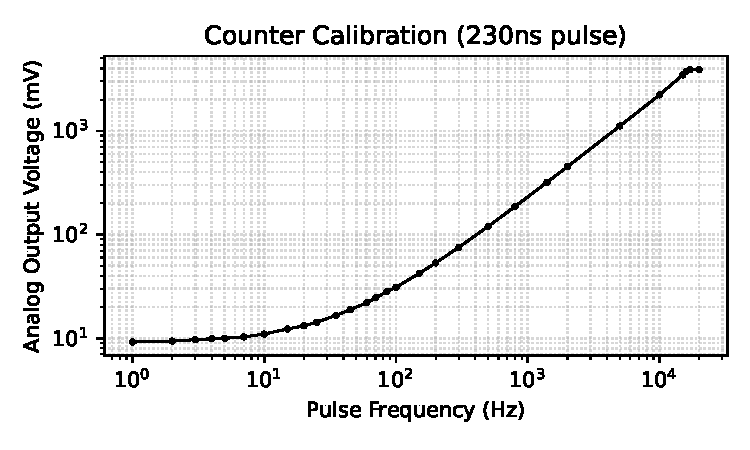
\includegraphics[width=0.6\textwidth]{../figures/task7_freq.pdf}
    \caption{Analog output voltage as a function of input pulse frequency plotted on a log-log scale, which elegantly linearizes the multi-decade sweep and visually highlights the strict bounds at \SI{45.45}{\hertz} and \SI{4}{\volt}.}
    \label{fig:task7}
\end{figure}

The linear region defines the calibration factor for the counter. A strict mathematical fit of the data between \SI{100}{\hertz} and \SI{10}{\kilo\hertz} yields a calibration factor $K \approx \SI{0.221}{\milli\volt\per\hertz}$, accompanied by an empirical DC offset of \SI{9.09}{\milli\volt}. The system exhibits two hard nonlinear boundaries. The high-frequency upper limit is characterized by a strict voltage saturation at approximately \SI{4}{\volt}. This is an electronic power rail limit, not an intrinsic frequency limit; the circuit operates on a \SI{5}{\volt} supply, and the operational amplifier suffers an approximate \SI{1}{\volt} internal dropout. 

Conversely, the lower frequency limit is dictated by the RC time constant of the continuous integrator, $T_{int} = \SI{1}{\mega\ohm} \times \SI{22}{\nano\farad} = \SI{22}{\milli\second}$. The corresponding decay limit $f_{int} = 1/T_{int} \approx \SI{45.45}{\hertz}$ perfectly matches the observed drop-off in voltage. During the initial measurements, the setup suffered severe low-frequency signal corruption. It was later realized that AC coupling on the oscilloscope was mistakenly utilized, causing the input capacitance to discharge through the internal $R_3$ resistor during the integration phase. Switching the channel to DC coupling immediately resolved the anomaly, yielding pristine measurements down to the intrinsic \SI{45.45}{\hertz} RC boundary.

\subsection{Temporal Delays and Convolution (Task 8)}

Figure~\ref{fig:task8} illustrates the analog coincidence output when sweeping a time delay between a short pulse (\SI{230}{\nano\second}) and a long pulse (\SI{2.25}{\micro\second}).

\begin{figure}[H]
    \centering
    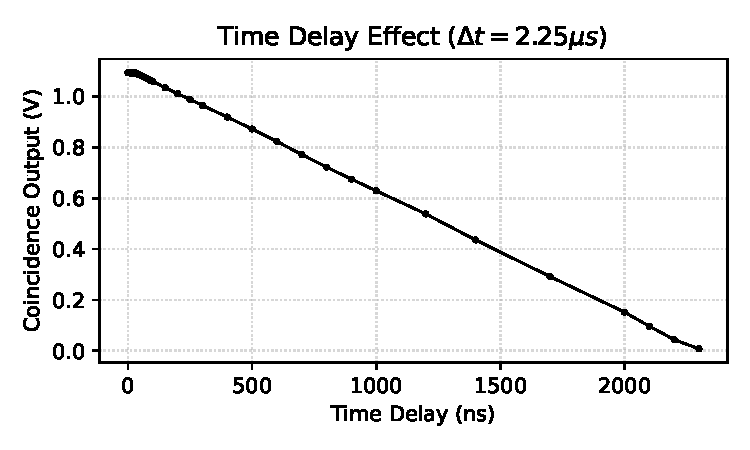
\includegraphics[width=0.6\textwidth]{../figures/task8_delay.pdf}
    \caption{Coincidence output as a function of temporal delay between the pulses.}
    \label{fig:task8}
\end{figure}

The resulting waveform represents the cross-correlation (convolution) of the two rectangular input pulses: $C(\tau) = \int V_{short}(t) V_{long}(t-\tau) dt$. Because the pulse widths are highly asymmetric (\SI{230}{\nano\second} and \SI{2.25}{\micro\second}), the convolution takes the mathematical shape of a wide trapezoid. The shortest measurable delay at which the coincidence signal noticeably begins to fall was empirically determined to be \SI{60}{\nano\second}, fundamentally characterizing the finite edge resolution and jitter of the AND gate electronics. The longest delay at which a coincidence was detected was \SI{2300}{\nano\second}, which aligns almost perfectly with the expected sum of the rectangular pulse widths ($\sim \SI{2.48}{\micro\second}$).

\subsection{Gated Detection and Random Coincidences (Tasks 9 and 10)}

Task 9 evaluated the system under an external sweep to confirm linear gated scaling (Figure~\ref{fig:task9}). To experimentally modulate the average count rate for these tests, one might classically assume that sweeping the frequency of a square wave to very low values would suffice. However, this method fundamentally fails: at low frequencies, the time between pulses exceeds the analog integrator's \SI{22}{\milli\second} RC time constant, causing the capacitor to discharge and severely corrupting the DC voltage reading. To elegantly solve this, the frequency was fixed at a high \SI{1}{\kilo\hertz} (safely above the \SI{45.45}{\hertz} RC cutoff), and the \textit{duty cycle} was swept instead. This successfully modulated the average single-photon count rate while completely dodging the integrator's aliasing limit.

\begin{figure}[H]
    \centering
    \begin{subfigure}{0.48\textwidth}
        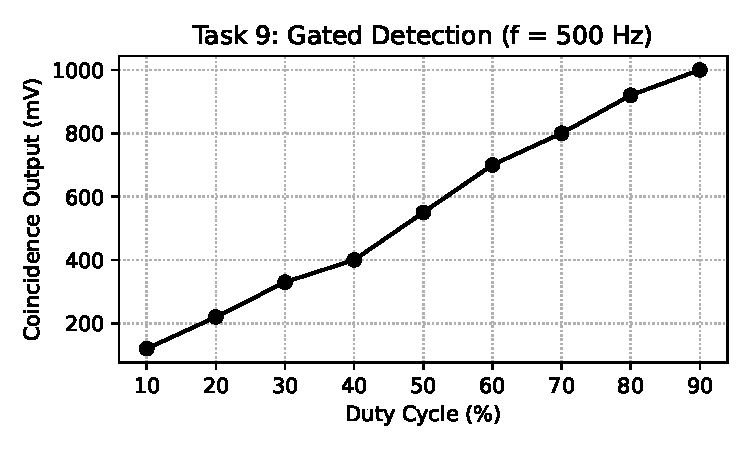
\includegraphics[width=\textwidth]{../figures/task9_duty.pdf}
    \end{subfigure}
    \begin{subfigure}{0.48\textwidth}
        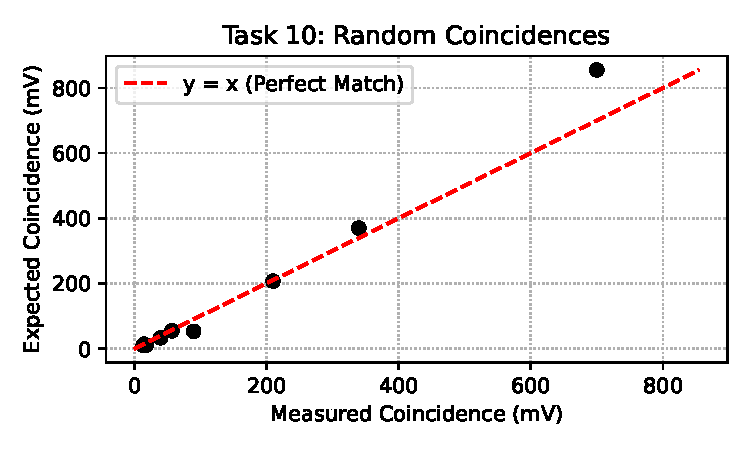
\includegraphics[width=\textwidth]{../figures/task10_rand.pdf}
    \end{subfigure}
    \caption{Left: Coincidence output versus gating duty cycle. Right: Measured versus expected random coincidences based on the classical probabilistic model.}
    \label{fig:task9}
\end{figure}

Task 10 quantified the statistics of purely random coincidences. The marginal singles voltages ($V_1, V_2$) were measured utilizing the short pulse setting ($\tau_{short} = \SI{230}{\nano\second}$), while the joint coincidence logic utilized the long pulse setting ($\tau_{long} = \SI{2.25}{\micro\second}$). Converting voltages to rates utilizes the calibration factor $K_{short} \approx \SI{0.221}{\milli\volt\per\hertz}$ and the DC baseline $V_{offset} \approx \SI{9.09}{\milli\volt}$, both derived directly from the linear regression of the analog counter sweep (Figure~\ref{fig:task7}). Physically, $K_{short}$ represents the intrinsic gain of the integrator (millivolts accumulated per \SI{1}{\hertz}), while $V_{offset}$ represents the innate quiescent baseline voltage of the operational amplifier when absolutely no pulses are arriving. 

The probability rate of random overlap for independent Poissonian sources is $c_{rand} = 2 \tau_{long} r_1 r_2$. Critically, the analog AND gate outputs a pulse whose average width is strictly $\tau_{long} / 2$ for overlapping uniform random pulses. Consequently, the analog integrator translates this to an expected joint voltage of $V_{joint} = c_{rand} \times (K_{long} / 2) + V_{offset} = \tau_{long} r_1 r_2 K_{long} + V_{offset}$. Because an integrator linearly accumulates voltage over time, the calibration factor scales strictly proportionally with the input pulse width; thus, $K_{long} = K_{short}(\tau_{long} / \tau_{short})$. Figure~\ref{fig:task9} (right) plots the measured joint voltage against this explicit theoretical expectation. The extraordinary linear agreement across two orders of magnitude strongly validates the stochastic overlap model and the temporal convolution mechanics of the AND gate. 

It is worth noting that a minor periodic background fluctuation in the counting baseline was initially attributed to the sinusoidal diurnal variation of ambient sunlight penetrating the laboratory shielding. However, this hypothesis is physically untenable, as the total measurement duration ($< 30$ minutes) constitutes a mathematically negligible fraction of the diurnal period. The fluctuation is therefore more appropriately attributed to transient stochastic environmental noise or passing cloud cover.

\section{Conclusion}
We have successfully characterized a Type-I BBO SPDC source. The physical extraction of the $\phi_0 \approx 3^\circ$ half-opening angle is validated by phase-matching theory. Electronic profiling of the coincidence logic quantified the RC integrator limit (\SI{45.45}{\hertz}) and op-amp saturation (\SI{4}{\volt}). Finally, the stochastic overlap model was verified to accurately predict the continuous random coincidence baseline.

\end{document}
